\documentclass[CJK]{beamer}
\usepackage{CJKutf8}
\usepackage{beamerthemesplit}
\usetheme{Malmoe}
\useoutertheme[footline=authortitle]{miniframes}
\usepackage{amsmath}
\usepackage{amssymb}
\usepackage{graphicx}
\usepackage{eufrak}
\usepackage{color}
\usepackage{slashed}
\usepackage{simplewick}
\usepackage{tikz}
\usepackage{ulem}
\usepackage{tcolorbox}
\graphicspath{{../figures/}}
%%figures
\def\lfig#1#2{\includegraphics[width=#1 in]{#2}}
\def\addfig#1#2{\begin{center}\includegraphics[width=#1 in]{#2}\end{center}}
\def\wulian{
\includegraphics[width=0.18in]{emoji_wulian.jpg}}
\def\bigwulian{
\includegraphics[width=0.35in]{emoji_wulian.jpg}}
\def\bye{
\includegraphics[width=0.18in]{emoji_bye.jpg}}
\def\bigbye{
\includegraphics[width=0.35in]{emoji_bye.jpg}}
\def\huaixiao{
\includegraphics[width=0.18in]{emoji_huaixiao.jpg}}
\def\bighuaixiao{
\includegraphics[width=0.35in]{emoji_huaixiao.jpg}}
\def\jianxiao{
\includegraphics[width=0.18in]{emoji_jianxiao.jpg}}
\def\bigjianxiao{
\includegraphics[width=0.35in]{emoji_jianxiao.jpg}}
%% colors
\def\blacktext#1{{\color{black}#1}}
\def\bluetext#1{{\color{blue}#1}}
\def\redtext#1{{\color{red}#1}}
\def\darkbluetext#1{{\color[rgb]{0,0.2,0.6}#1}}
\def\skybluetext#1{{\color[rgb]{0.2,0.7,1.}#1}}
\def\cyantext#1{{\color[rgb]{0.,0.5,0.5}#1}}
\def\greentext#1{{\color[rgb]{0,0.7,0.1}#1}}
\def\darkgray{\color[rgb]{0.2,0.2,0.2}}
\def\lightgray{\color[rgb]{0.6,0.6,0.6}}
\def\gray{\color[rgb]{0.4,0.4,0.4}}
\def\blue{\color{blue}}
\def\red{\color{red}}
\def\green{\color{green}}
\def\darkgreen{\color[rgb]{0,0.4,0.1}}
\def\darkblue{\color[rgb]{0,0.2,0.6}}
\def\skyblue{\color[rgb]{0.2,0.7,1.}}
%%control
\def\be{\begin{equation}}
\def\ee{\nonumber\end{equation}}
\def\bea{\begin{eqnarray}}
\def\eea{\nonumber\end{eqnarray}}
\def\bch{\begin{CJK}{UTF8}{gbsn}}
\def\ech{\end{CJK}}
\def\bitem{\begin{itemize}}
\def\eitem{\end{itemize}}
\def\bcenter{\begin{center}}
\def\ecenter{\end{center}}
\def\bex{\begin{minipage}{0.2\textwidth}
\includegraphics[width=0.6in]{jugelizi.png}\end{minipage}\begin{minipage}{0.76\textwidth}}
\def\eex{\end{minipage}}
\def\chtitle#1{\frametitle{\bch#1\ech}}
\def\bmat#1{\left(\begin{array}{#1}}
\def\emat{\end{array}\right)}
\def\bcase#1{\left\{\begin{array}{#1}}
\def\ecase{\end{array}\right.}
\def\bmini#1{\begin{minipage}{#1\textwidth}}
\def\emini{\end{minipage}}
\def\tbox#1{\begin{tcolorbox}#1\end{tcolorbox}}
\def\pfrac#1#2#3{\left(\frac{\partial #1}{\partial #2}\right)_{#3}}
%%symbols
\def\sone{$\star$}
\def\stwo{$\star\star$}
\def\sthree{$\star\star\star$}
\def\sfour{$\star\star\star\star$}
\def\sfive{$\star\star\star\star\star$}
\def\rint{{\int_\leftrightarrow}}
\def\roint{{\oint_\leftrightarrow}}
\def\stdHf{{\textit{\r H}_f}}
\def\deltaH{{\Delta \textit{\r H}}}
\def\ii{{\dot{\imath}}}
\def\skipline{{\vskip0.1in}}
\def\skiplines{{\vskip0.2in}}
\def\lagr{{\mathcal{L}}}
\def\hamil{{\mathcal{H}}}
\def\vecv{{\mathbf{v}}}
\def\vecx{{\mathbf{x}}}
\def\vecy{{\mathbf{y}}}
\def\veck{{\mathbf{k}}}
\def\vecp{{\mathbf{p}}}
\def\vecn{{\mathbf{n}}}
\def\vecA{{\mathbf{A}}}
\def\vecP{{\mathbf{P}}}
\def\vecsigma{{\mathbf{\sigma}}}
\def\hatJn{{\hat{J_\vecn}}}
\def\hatJx{{\hat{J_x}}}
\def\hatJy{{\hat{J_y}}}
\def\hatJz{{\hat{J_z}}}
\def\hatj#1{\hat{J_{#1}}}
\def\hatphi{{\hat{\phi}}}
\def\hatq{{\hat{q}}}
\def\hatpi{{\hat{\pi}}}
\def\vel{\upsilon}
\def\Dint{{\mathcal{D}}}
\def\adag{{\hat{a}^\dagger}}
\def\bdag{{\hat{b}^\dagger}}
\def\cdag{{\hat{c}^\dagger}}
\def\ddag{{\hat{d}^\dagger}}
\def\hata{{\hat{a}}}
\def\hatb{{\hat{b}}}
\def\hatc{{\hat{c}}}
\def\hatd{{\hat{d}}}
\def\hatN{{\hat{N}}}
\def\hatH{{\hat{H}}}
\def\hatp{{\hat{p}}}
\def\Fup{{F^{\mu\nu}}}
\def\Fdown{{F_{\mu\nu}}}
\def\newl{\nonumber \\}
\def\vece{\mathrm{e}}
\def\calM{{\mathcal{M}}}
\def\calT{{\mathcal{T}}}
\def\calR{{\mathcal{R}}}
\def\barpsi{\bar{\psi}}
\def\baru{\bar{u}}
\def\barv{\bar{\upsilon}}
\def\qeq{\stackrel{?}{=}}
\def\torder#1{\mathcal{T}\left(#1\right)}
\def\rorder#1{\mathcal{R}\left(#1\right)}
\def\contr#1#2{\contraction{}{#1}{}{#2}#1#2}
\def\trof#1{\mathrm{Tr}\left(#1\right)}
\def\trace{\mathrm{Tr}}
\def\comm#1{\ \ \ \left(\mathrm{used}\ #1\right)}
\def\tcomm#1{\ \ \ (\text{#1})}
\def\slp{\slashed{p}}
\def\slk{\slashed{k}}
\def\calp{{\mathfrak{p}}}
\def\veccalp{\mathbf{\mathfrak{p}}}
\def\Tthree{T_{\tiny \textcircled{3}}}
\def\pthree{p_{\tiny \textcircled{3}}}
\def\dbar{{\,\mathchar'26\mkern-12mu d}}
\def\erf{\mathrm{erf}}
\def\const{\mathrm{constant}}
\def\pheat{\pfrac p{\ln T}V}
\def\vheat{\pfrac V{\ln T}p}
%%units
\def\fdeg{{^\circ \mathrm{F}}}
\def\cdeg{^\circ \mathrm{C}}
\def\atm{\,\mathrm{atm}}
\def\angstrom{\,\text{\AA}}
\def\SIL{\,\mathrm{L}}
\def\SIkm{\,\mathrm{km}}
\def\SIyr{\,\mathrm{yr}}
\def\SIGyr{\,\mathrm{Gyr}}
\def\SIV{\,\mathrm{V}}
\def\SImV{\,\mathrm{mV}}
\def\SIeV{\,\mathrm{eV}}
\def\SIkeV{\,\mathrm{keV}}
\def\SIMeV{\,\mathrm{MeV}}
\def\SIGeV{\,\mathrm{GeV}}
\def\SIcal{\,\mathrm{cal}}
\def\SIkcal{\,\mathrm{kcal}}
\def\SImol{\,\mathrm{mol}}
\def\SIN{\,\mathrm{N}}
\def\SIHz{\,\mathrm{Hz}}
\def\SIm{\,\mathrm{m}}
\def\SIcm{\,\mathrm{cm}}
\def\SIfm{\,\mathrm{fm}}
\def\SImm{\,\mathrm{mm}}
\def\SInm{\,\mathrm{nm}}
\def\SImum{\,\mathrm{\mu m}}
\def\SIJ{\,\mathrm{J}}
\def\SIW{\,\mathrm{W}}
\def\SIkJ{\,\mathrm{kJ}}
\def\SIs{\,\mathrm{s}}
\def\SIkg{\,\mathrm{kg}}
\def\SIg{\,\mathrm{g}}
\def\SIK{\,\mathrm{K}}
\def\SImmHg{\,\mathrm{mmHg}}
\def\SIPa{\,\mathrm{Pa}}

\title{Cosmic Microwave Background}
\author{Zhiqi Huang}
\institute{Sun Yat-sen University}
\date{June 12, 2017}


\begin{document}

\begin{frame}
  \bch
  \bcenter
      {\Huge 宇宙背景微波辐射}

      \addfig{1.8}{planck_fullsky.jpg}
      
      {\Large 黄志琦}

      \skipline
      
      中山大学物理与天文学院 
      
      {2017年6月11日}
      \ecenter
      \ech
\end{frame}


\begin{frame}
\chtitle{欢迎报考中山大学}
\bch
\centering

\lfig{0.2}{SYSUlogo.jpg}中山大学珠海校区 物理与天文学院

\addfig{3}{schoolprofile.png}

{\large \bf http://spa.sysu.edu.cn}

\ech
\end{frame}

\begin{frame}
\chtitle{欢迎报考中山大学}
\addfig{2.5}{spascan.jpg}
\end{frame}


\begin{frame}
\chtitle{欢迎报考中山大学}
\addfig{3.}{SYSU_campus.jpg}
\end{frame}


\begin{frame}
\chtitle{现代物理学未解决的基础理论问题都和宇宙学息息相关}
\centering
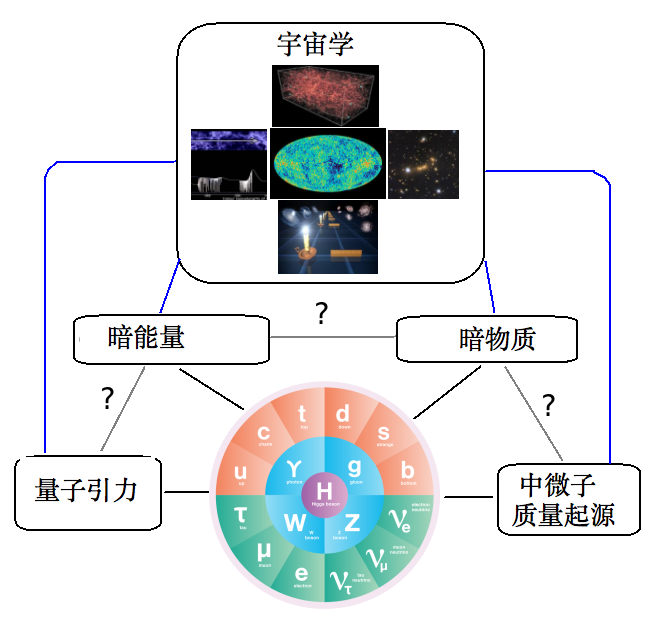
\includegraphics[width=3.in]{cosmo_value1.png}
\end{frame}


\begin{frame}
\chtitle{内容摘要}
\centering
\bch
\bitem
\item{宇宙的尺度和构成}
\item{宇宙背景微波辐射}
\item{第一推动力从何而来}
\item{未来会怎样}
  \eitem
  \ech
\end{frame}

\section{Size of Universe}
\begin{frame}
  \chtitle{形象地丈量长度的办法:熟知的速度$\times$时间}
  \bch
  \bitem
\item{从教学楼到兵哥食坊,大概5分钟步行路程。}
\item{从学校到扬名海底捞,大概20分钟车程。}
\item{从珠海到北京全聚德,大概4小时飞机。}
  \eitem

  
  \ech
\end{frame}

\begin{frame}
  \chtitle{从中国到美国}
  \bch
  飞机从中国飞到美国,大概需要十几小时。
  \addfig{1.5}{plane.jpg}
  而跑得最快的光,大概只需要几十毫秒。
  \addfig{1.5}{light.jpg}
  \ech
\end{frame}


\begin{frame}
  \chtitle{宇宙有多大:地月距离}
  \bch

  \addfig{3}{earth_to_moon.jpg}
 \bcenter 
  从地球到月球,光要跑大约1秒。
  \ecenter
  \ech
\end{frame}


\begin{frame}
  \chtitle{宇宙有多大:太阳系的行星}
  \bch
  \addfig{3.8}{solar-system.jpg}
 \bcenter 
 从太阳到地球,光要跑大约8分钟,即使跑到最远的海王星也只要大概几个小时。
  \ecenter
  \ech
\end{frame}


\begin{frame}
  \chtitle{宇宙有多大:附近的其他“太阳系”}
  \bch
  \addfig{3.3}{sun_neighbors.png}
 \bcenter 
 光跑到离太阳最近的另一个”太阳“(恒星)大概需要4年。
  \ecenter
  \ech
\end{frame}


\begin{frame}
  \chtitle{宇宙有多大:银河系}
  \bch
  \bmini{0.7}
  \addfig{2.6}{Milkway.jpg}
  \emini
  \bmini{0.26}
  银河系里大概有一千亿个“太阳”(恒星)

  \skipline
  
  光从银河系一边跑到另一边要10万年以上。
  \emini

  {\scriptsize 如果把太阳系比做一枚硬币,银河系大概有中国版图那么大。}

  \ech
\end{frame}


\begin{frame}
  \chtitle{宇宙有多大:其他星系}
  \bch
  \bmini{0.7}
  \addfig{2.6}{galaxies.jpg}
  \emini
  \bmini{0.26}
  可观测宇宙中大概有一千亿个”银河系“(星系)

  \skipline
  
  我们看到的来自可观测宇宙的“边缘”的光大概已经跑了一百三十多亿年。
  \emini

  {\scriptsize 如果把银河系比做一块瓷砖,可观测宇宙大概有中国版图那么大。}
  
  \ech
\end{frame}

\begin{frame}
  \chtitle{先牛时代}
  \bch
  在牛顿提出(?)万有引力之前,宇宙学基本是一个宗教和哲学问题。
  \ech
\end{frame}


\begin{frame}
\chtitle{佛教}
\bch
\begin{minipage}{0.45\textwidth}
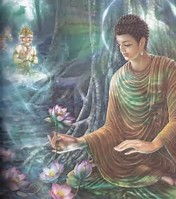
\includegraphics[width=1.6in]{buddist.jpg}
\end{minipage}
\begin{minipage}{0.45\textwidth}
{\Large 一花一叶一世界}
\end{minipage}
\ech
\end{frame}


\begin{frame}
\chtitle{道教}
\bch
\begin{minipage}{0.45\textwidth}

\includegraphics[width=1.6in]{laozi.jpeg}
\end{minipage}
\begin{minipage}{0.45\textwidth}
{\Large 天下万物生于有,有生于无}
\end{minipage}
\ech
\end{frame}


\begin{frame}
\chtitle{远古神话}
\bch

\bmini{0.42}

\includegraphics[height=2in]{pangu1.jpg}
\emini
\bmini{0.54}

\includegraphics[height=2in]{pangu.jpg}
\emini

\ech
\end{frame}

\begin{frame}
\chtitle{基督教}
\bch
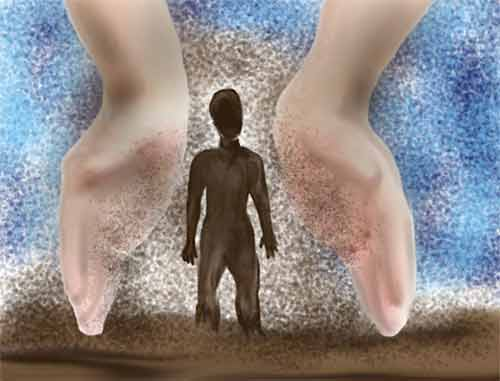
\includegraphics[height=1.6in]{createhuman.jpg}
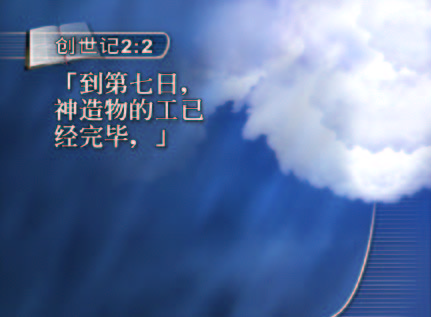
\includegraphics[height=1.6in]{creation.jpg}
\ech
\end{frame}

\begin{frame}
  \chtitle{后来}
  \bch
  {\Large
  大boss牛顿出现了……}
  \ech
\end{frame}


\begin{frame}
  \chtitle{万有引力定律}
  \bch
  \addfig{3.2}{NewtonApple.jpg}
  \ech
\end{frame}


\begin{frame}
  \chtitle{正如大多数励志科学家故事}
  \bch
  \addfig{2.2}{bucunzai.png}
  \ech
\end{frame}

\begin{frame}
  \chtitle{胡牛之争}
  \bch

  根据已经公开出版的牛顿信件{\scriptsize (Page 297 in H W Turnbull (ed.), Correspondence of Isaac Newton, Vol 2 (1676-1687), (Cambridge University Press, 1960), document \#235, 24 November 1679.)}:
  
  {\blue 在牛顿发表万有引力定律之前,胡克(就是玩弹簧的那位dalao)在和牛顿的信件中不仅提到了引力的平方反比律,而且提出了天体运动是由引力提供向心力所致。}

  \addfig{2}{huniu.png}
  \ech
\end{frame}

\begin{frame}
  \chtitle{拉普拉斯妖——牛顿力学的辉煌时期}
  \addfig{3}{Laplace.jpg}

  \bch
  似乎除了牛顿提到的“上帝之第一推动”,其余问题都解决了。
  \ech
\end{frame}


\begin{frame}
  \chtitle{然后}
  \bch
  随着观测技术的不断进步,问题又来了……
  \ech
\end{frame}


\begin{frame}
  \chtitle{牛顿引力的问题}
  \bch
  \bmini{0.45}
  \addfig{1.8}{MercuryProcession.jpg}
  \emini
  \bmini{0.5}
  \bitem
\item[A]{水星进动}
\item[B]{光线经过恒星附近时的弯曲}
\item[C]{星系外围恒星运动速度}
\item[D]{超新星测距得出宇宙加速膨胀}
  \eitem
  \emini
  \ech
\end{frame}

\begin{frame}
  \chtitle{广义相对论}
  \bch
  \bmini{0.42}
  \addfig{0.8}{einstein.jpeg}

  
  \addfig{1.6}{lightcurve.jpg}
  \emini
  \bmini{0.54}
  大概100年前,dalao爱因斯坦说:

  \skipline
  
  {\Large \bf 引力?不存在的。只不过时空有些弯曲而已…}

  \skiplines
  
  \bitem
\item[A]{\sout{水星进动}}
\item[B]{\sout{光线经过恒星附近时的弯曲}}
\item[C]{星系外围恒星运动速度}
\item[D]{超新星测距得出宇宙加速膨胀}  
  \eitem
  \emini
  \ech
\end{frame}

\begin{frame}
  \chtitle{宇宙学基本模型“解决”了剩下两个问题}
  \bch
  \bmini{0.5}
  \lfig{2}{pie.png}
  \emini
  \bmini{0.45}
  \bitem
\item{69\%暗能量 $\Rightarrow$ 宇宙加速膨胀}
\item{26\%暗物质 $\Rightarrow$ 星系外围恒星运动}
\item{5\%已知物质}
  \eitem
  \emini
  \ech
\end{frame}

\section{CMB}

\begin{frame}
  \chtitle{现代版的“混沌初开”}
  \bch
  \bitem
\item{宇宙一开始是很热的“一片混沌”
\addfig{2}{hundun.jpg}
}
\item{温度随着宇宙膨胀而降低}
\item{当温度降到$3000\SIK$(大概太阳表面温度的一半)时,“混沌初开”,宇宙变得透明}
  \eitem

  \wulian 怎么听着跟盘古的故事那么像
  
  \ech
\end{frame}

\begin{frame}
  \chtitle{宇宙背景微波辐射(CMB)的预言}
  \bch
  \addfig{3.2}{last_scattering.jpg}
  \ech
\end{frame}


\begin{frame}
  \chtitle{CMB的预言和发现}
  \bch
  \bitem
\item{1950年, Alpher 和 Herman预言了CMB:黑体谱,温度大约几$K$}
\item{1964年, Penzias 和 Wilson 在射电望远镜噪声中意外发现了约$3\SIK$的背景辐射}
\item{1989年11月, COBE卫星带着测量CMB的使命升空}
\item{ \bmini{0.54} \lfig{2}{COBECMB.png} \emini
  \bmini{0.42}1990年1月的美国天文学会一次会议上,J. C. Mather通过一张幻灯片展示观测到的CMB谱和黑体谱完全吻合时,全场响起了热烈的掌声\emini
}  
  \eitem

  \ech
\end{frame}

\begin{frame}
  \chtitle{CMB在各个方向上温度非常均匀}
  \bch
  \addfig{3}{uniform_cmb_sphere.png}
  \ech
\end{frame}


\begin{frame}
  \chtitle{虽然非常均匀,但在各个方向上还是有大概十万分之一的起伏}
  \bch
  \addfig{2}{cmb_sphere.jpg}
  \bcenter
  
  把平均温度($2.72585\SIK$)减掉后的CMB温度图
  \ecenter
  \ech
\end{frame}

\section{Initial Conditions}
\begin{frame}
  \chtitle{我们通常喜欢像画世界地图一样把天球展开到一个平面上}
  \bch
  \addfig{3}{wmap_fullsky.jpg}
  CMB在各个方向上的温度有大概十万分之一的起伏。
  \ech
\end{frame}


\begin{frame}
  \chtitle{对极早期宇宙的猜测}
  \bch
  即使物理规律相同,不同的初始条件也会演化出不同的结果。

  \skiplines

  那么,宇宙的初始条件是什么呢?
  \ech
\end{frame}


\begin{frame}
\chtitle{真空不空}
\bch
\begin{minipage}{0.5\textwidth}
场无处不在
\skipline
每种场对应一种粒子(或一对正反粒子)。例如电磁场对应光子,Dirac场对应正负电子。
\end{minipage}
\begin{minipage}{0.4\textwidth}
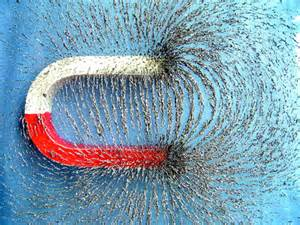
\includegraphics[width=1.5in]{magnet.jpeg}
\end{minipage}
\ech
\end{frame}

\begin{frame}
\chtitle{物理真空的定义}
\bch
\begin{minipage}{0.35\textwidth}
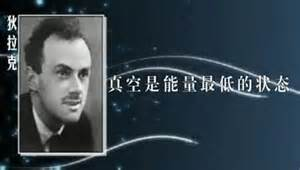
\includegraphics[width=1.2in]{vacuum.jpeg}
\end{minipage}\begin{minipage}{0.55\textwidth}
当所有场都处于最低能量态(即0个粒子的态)的时候,就是物理上定义的真空。
\end{minipage}

\skipline
\begin{equation}
\begin{array}{ccclr}
- & - & - & \mathrm{3\ particles} &\\
- & - & - & \mathrm{2\ particles}&\\
- & - & - & \mathrm{1\ particle} &\\
- & - & - & \mathrm{0\ particles}& \rightarrow {\bf \rm vacuum}\\ 
{\rm field\ A} & {\rm field\ B} & {\rm field\ C}
\end{array} \nonumber
\end{equation}
{\scriptsize
注:本图的上面几行仅为示意,实际上一个粒子可以拥有比两个粒子更多的能量。
}

\ech
\end{frame}

\begin{frame}
\chtitle{“无中生有”没有你想象得那么容易}
\bch

无论是经典理学还是量子力学都要求能量守恒。从最低能态变到不是最低的能态,势必破坏能量守恒。

\skipline
所以正常情况下真空里什么都不会产生!

\ech
\end{frame}

\begin{frame}
\chtitle{这个道理很显然}
\bch

\addfig{3}{geyoutang.jpg}

这样是不会发财的

\ech
\end{frame}


\begin{frame}
  \bch
  \chtitle{当然,也有例外情况}
  \addfig{3}{fangjia.jpg}
  
  例如: 你家房子地段好,坐看房价起飞
\ech
\end{frame}

\begin{frame}
\chtitle{粒子场住的“房子”}
\bch
各种粒子的场都“住”在四维时空里。如果时空结构发生剧烈变化,就能“无中生有”。

\skipline

基于这种想法的理论:
\begin{itemize}
\item{霍金的黑洞蒸发理论}
\item{宇宙早期暴涨(Inflation)理论}
\end{itemize}
\ech
\end{frame}

\begin{frame}
\chtitle{等一下,我还有问题}
\bch
\begin{itemize}
\item{早期宇宙时空{\blue \large 为何会暴涨}?}
\item{就算承认早期宇宙有个暴涨过程,不是说量子场论和广义相对论还没统一吗?那{\blue \large 怎么计算}时空剧烈变化时的各种量子场的行为?}
\end{itemize}
\ech
\end{frame}

\begin{frame}
\chtitle{为何暴涨}
\bch
{\blue 为何暴涨}的问题,100年前已经被{\blue 爱因斯坦解决了}:

\begin{minipage}{0.45\textwidth}
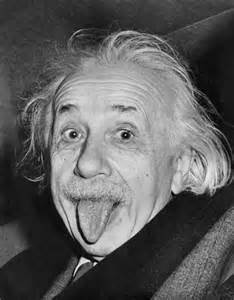
\includegraphics[width=1.2in]{einstein.jpeg}
\end{minipage}
\begin{minipage}{0.45\textwidth}
$$ M_p^2 G^{\mu\nu} =  T^{\mu\nu} - \rho_{\rm vacuum} g^{\mu\nu} $$
广义相对论里的Einstein方程:真空能和标量场的势能都具有排斥作用会使空间加速膨胀。

\end{minipage}
\ech
\end{frame}

\begin{frame}
\chtitle{怎么计算弯曲时空里的量子场}
\bch
关于{\blue 怎么计算},有一个好消息和一个坏消息。
\ech
\end{frame}

\begin{frame}
\chtitle{好消息和坏消息}
\bch
\begin{minipage}{0.6\textwidth}
坏消息:我们无法从第一原理出发计算黑洞蒸发或者早期宇宙的时空暴涨。
\end{minipage}
\begin{minipage}{0.3\textwidth}

\includegraphics[width=0.8in]{baozou_haha.png}
\end{minipage}

\skipline
\skipline

好消息:霍金以及一批俄罗斯科学家发展起来了一种在特殊情况下可以从平直时空外推到弯曲时空的计算方法。
\ech
\end{frame}


\begin{frame}
\chtitle{有趣的是:这套计算方法管用}
\bch
现代宇宙学的大量观测验证了这套计算方法非常管用。

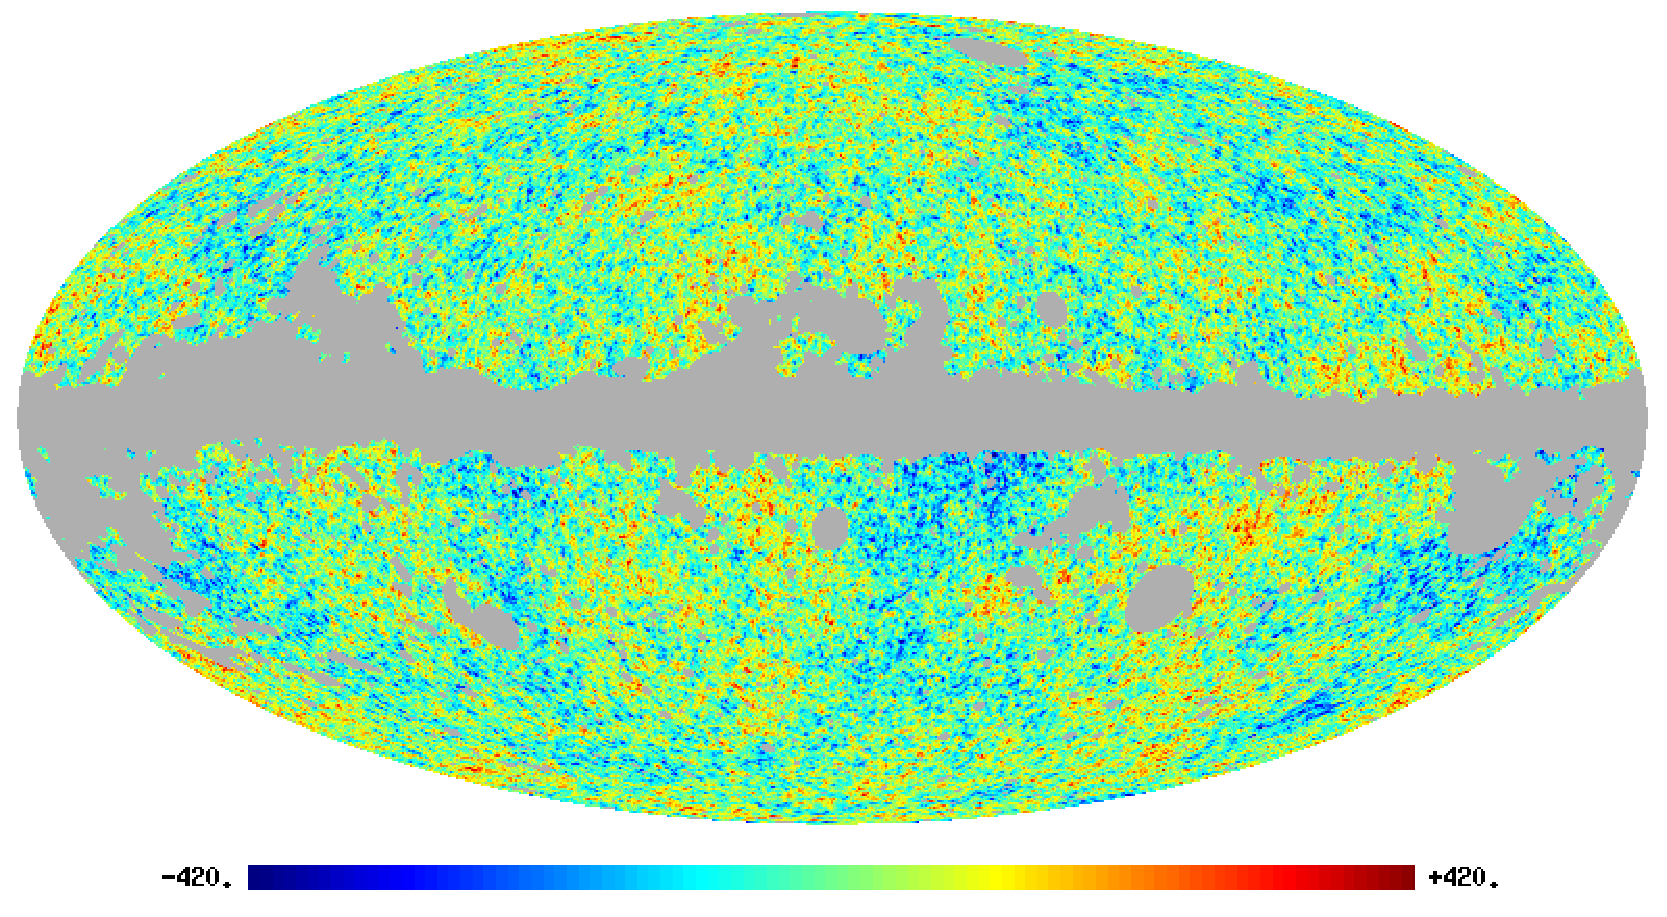
\includegraphics[width=1.5in]{planck_masked.pdf}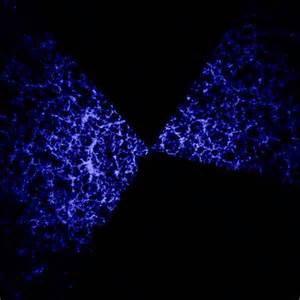
\includegraphics[width=1.in]{sdss.jpeg}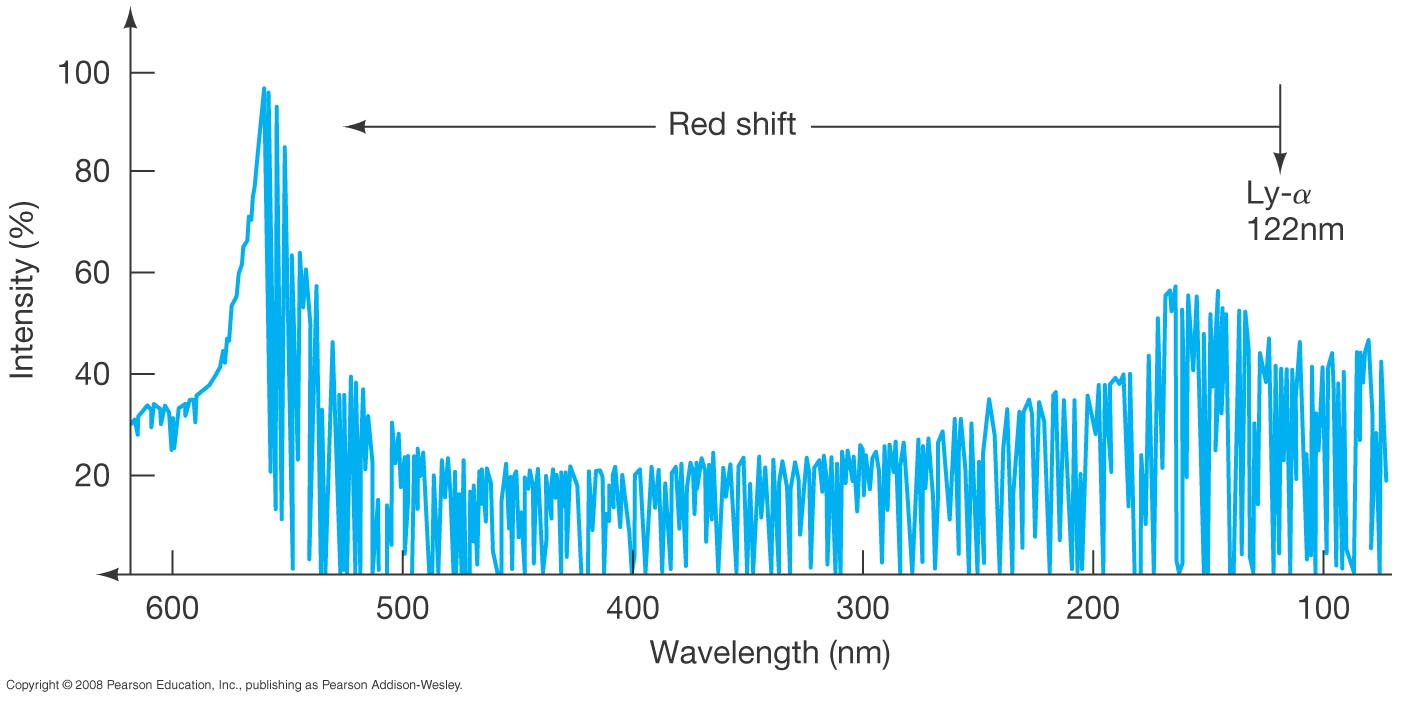
\includegraphics[width=1.5in]{lymanalpha.jpg}

现在的宇宙学标准模型里只有6个自由参数。我们迄今已经检查了数百亿个观测数据,没有发现任何和理论预言矛盾的地方!

\skipline
\skipline
那么,这套计算方法为什么管用呢?
\ech
\end{frame}


\begin{frame}
\chtitle{物理学革命呼之欲出?}
\bch
\begin{minipage}{0.6\textwidth}
谁知道它为什么管用!
\end{minipage}
\begin{minipage}{0.3\textwidth}

\includegraphics[width=0.8in]{baozou_haha.png}
\end{minipage}

\skipline
\skipline
\skipline
\skipline
还记得一百年前大家知道怎么算波尔半径,光电效应等等,却不知道为什么能这样算的情形么?
\ech
\end{frame}

%\begin{frame}
%\chtitle{宇宙学标准模型的概貌}
%\bch
%\begin{itemize}
%\item{真空暴涨,宇宙加速膨胀(约持续$\sim 10^{-35}$s)}
%\item{暴涨场衰变成其他场,热宇宙诞生,失去了真空能推斥力,宇宙开始减速膨胀并随着膨胀而冷却}
%\item{标准模型粒子形成(这时宇宙年龄才约$1$s),这时因为温度极高,原子还都处于电离状态,自由电子到处和光子发生散射,使得宇宙非常地“不透明”。}
%\item{宇宙冷却到大概$3000$K的时候,因宇宙中的光子能量不够电离氢原子,大部分自由电子都被氢原子核俘获。从此刻起光子即能自由穿行而不被自由电子散射。宇宙此时变得“透明”。此时宇宙的年龄约为几十万年。}
%\item{宇宙冷却后的膨胀过程和宇宙的具体组成有关,经过观测我们推测宇宙中有暗物质(和普通物质一样起到吸引作用,使得宇宙的膨胀慢下来)和暗能量(类似真空能有排斥作用,使宇宙最近又开始加速膨胀)。现在宇宙的年龄是一百三十多亿年。}
%\end{itemize}
%\ech
%\end{frame}

%\begin{frame}
%\chtitle{宇宙背景微波辐射(CMB)}
%\bch
%我们用电磁波观测能看到的最早的宇宙,是刚开始变成透明时的宇宙。那时的宇宙的光子自由穿行一百三十多亿年后被我们在地球上接收到。因为宇宙变透明后一直都在膨胀,这些光子波长被拉长后能量降低,到现在大约只有3K了。

%\skipline
%这个大约为3K的来自四面八方的光子,就是宇宙背景微波辐射(Cosmic Microwave Background)。
%\ech
%\end{frame}


%\begin{frame}
%\chtitle{CMB在各个方向上的温度起伏}
%\bch
%这个背景温度的数值对我们而言用处不大,有用的信息包含在各个方向的CMB的温度起伏中。这些起伏非常小,大概是$0.1$mK的量级。

%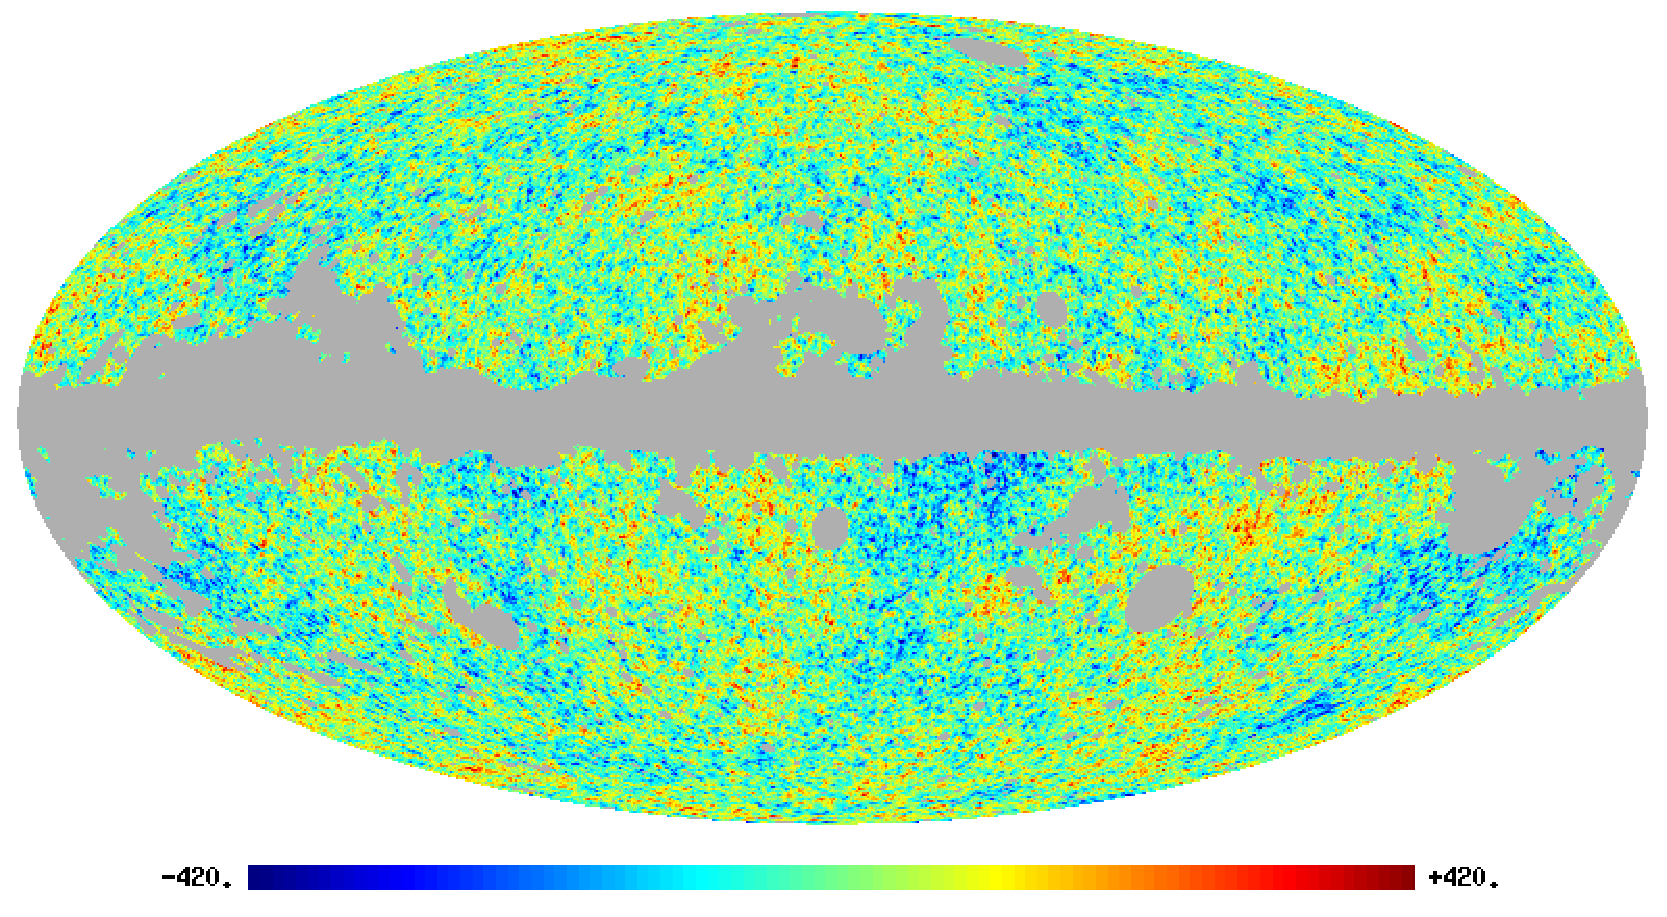
\includegraphics[width=3in]{planck_masked.pdf}
%\ech
%\end{frame}

\begin{frame}
\chtitle{CMB的统计性质}
\bch
CMB温度起伏的根源可以一直追溯到最开始的真空暴涨。

\tbox{真空态的统计性质 $\Rightarrow$ CMB的各种统计性质}

\skipline
最简单的,例如我们可以固定一个角度$\theta$,然后计算夹角为$\theta$的任意两个方向的CMB温度起伏的乘积的统计平均(这称为两点关联函数)。
\ech
\end{frame}

\begin{frame}
\chtitle{CMB的温度场两点关联函数测量}
\bch
习惯上我们喜欢讨论$C(\theta)$的勒让德变换$\mathcal{D}_\ell$。只要记住小的$\ell$对应大的$\theta$,这完全不影响我们理解下图:
  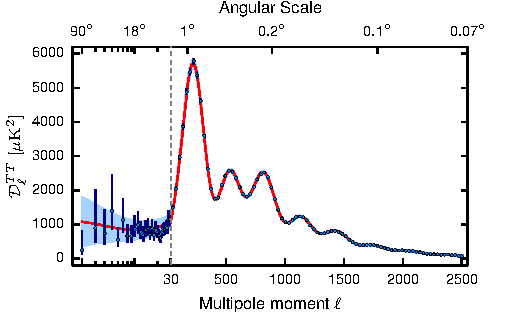
\includegraphics[width=3.5in]{planck2014_TT_Dl_NORES_bin30_w88mm.pdf}

  Planck卫星观测到的CMB温度场两点关联函数跟理论的比较。
\ech
\end{frame}

\begin{frame}
\chtitle{CMB的极化度测量}
\bch
实际上,对CMB我们不仅能观测它的温度,还能观测它的极化程度。(每个光子都有两个极化方向可以选择。)


这又提供了一种检验理论的办法。
\ech
\end{frame}


\begin{frame}
  \chtitle{Planck观测到的CMB温度场和极化场的两点关联函数}
  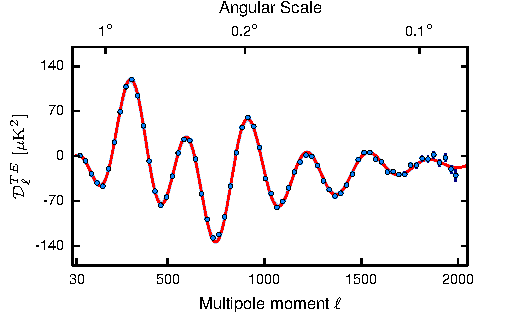
\includegraphics[width=3.5in]{planck2014_TE_Dl_NORES_bin30_w88mm.pdf}
\end{frame}

\begin{frame}
  \chtitle{Planck观测到的CMB极化场自身的两点关联函数}
  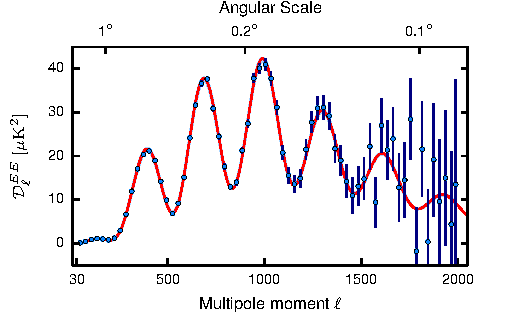
\includegraphics[width=3.5in]{planck2014_EE_Dl_NORES_bin30_w88mm.pdf}
\end{frame}


\begin{frame}
  \chtitle{不喜欢关联函数?没关系,我们可以把温度场图进行直接叠加。}
  \centering{
    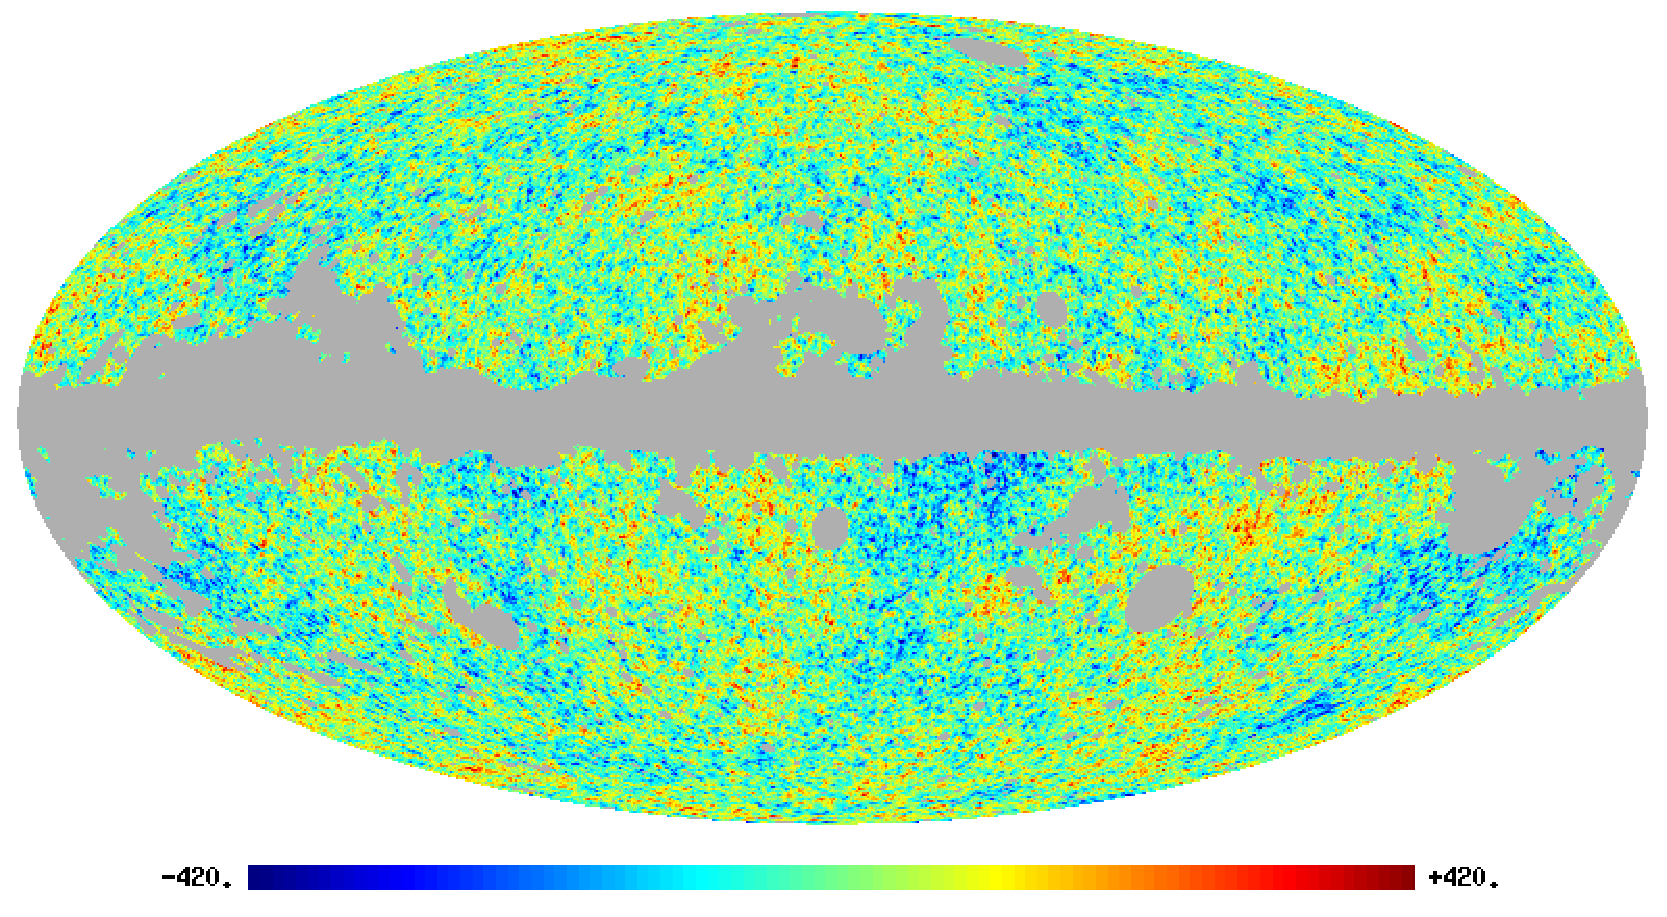
\includegraphics[width = 2.in]{planck_masked.pdf}}
  
  {\hskip 0.2in} {\scriptsize unoriented stacking}     {\hskip 0.65in} {\scriptsize oriented stacking (Bond, Frolov, Huang)}
            
  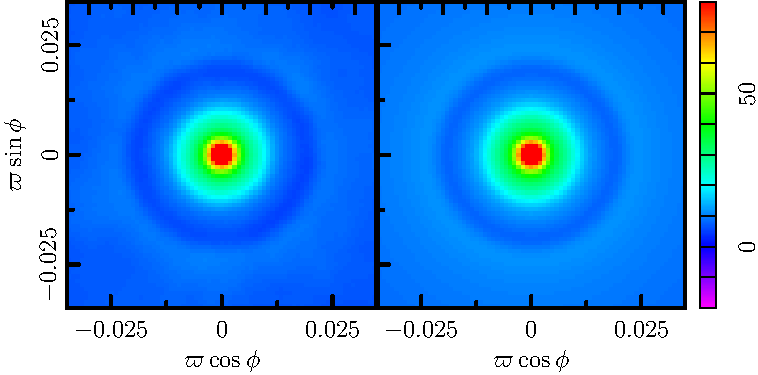
\includegraphics[width = 2in]{ors_T_on_Tmax_unoriented.pdf}  
  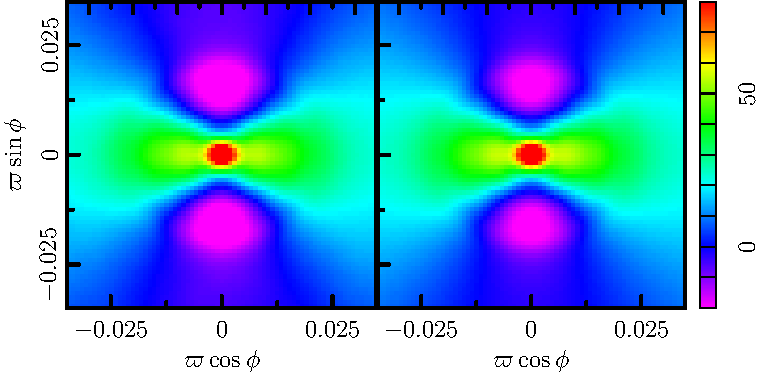
\includegraphics[width = 2in]{ors_T_on_Tmax_oriented.pdf}
\end{frame}

%\begin{frame}
%  \frametitle{The CMB Polarization Anisotropy Map from Planck}
%  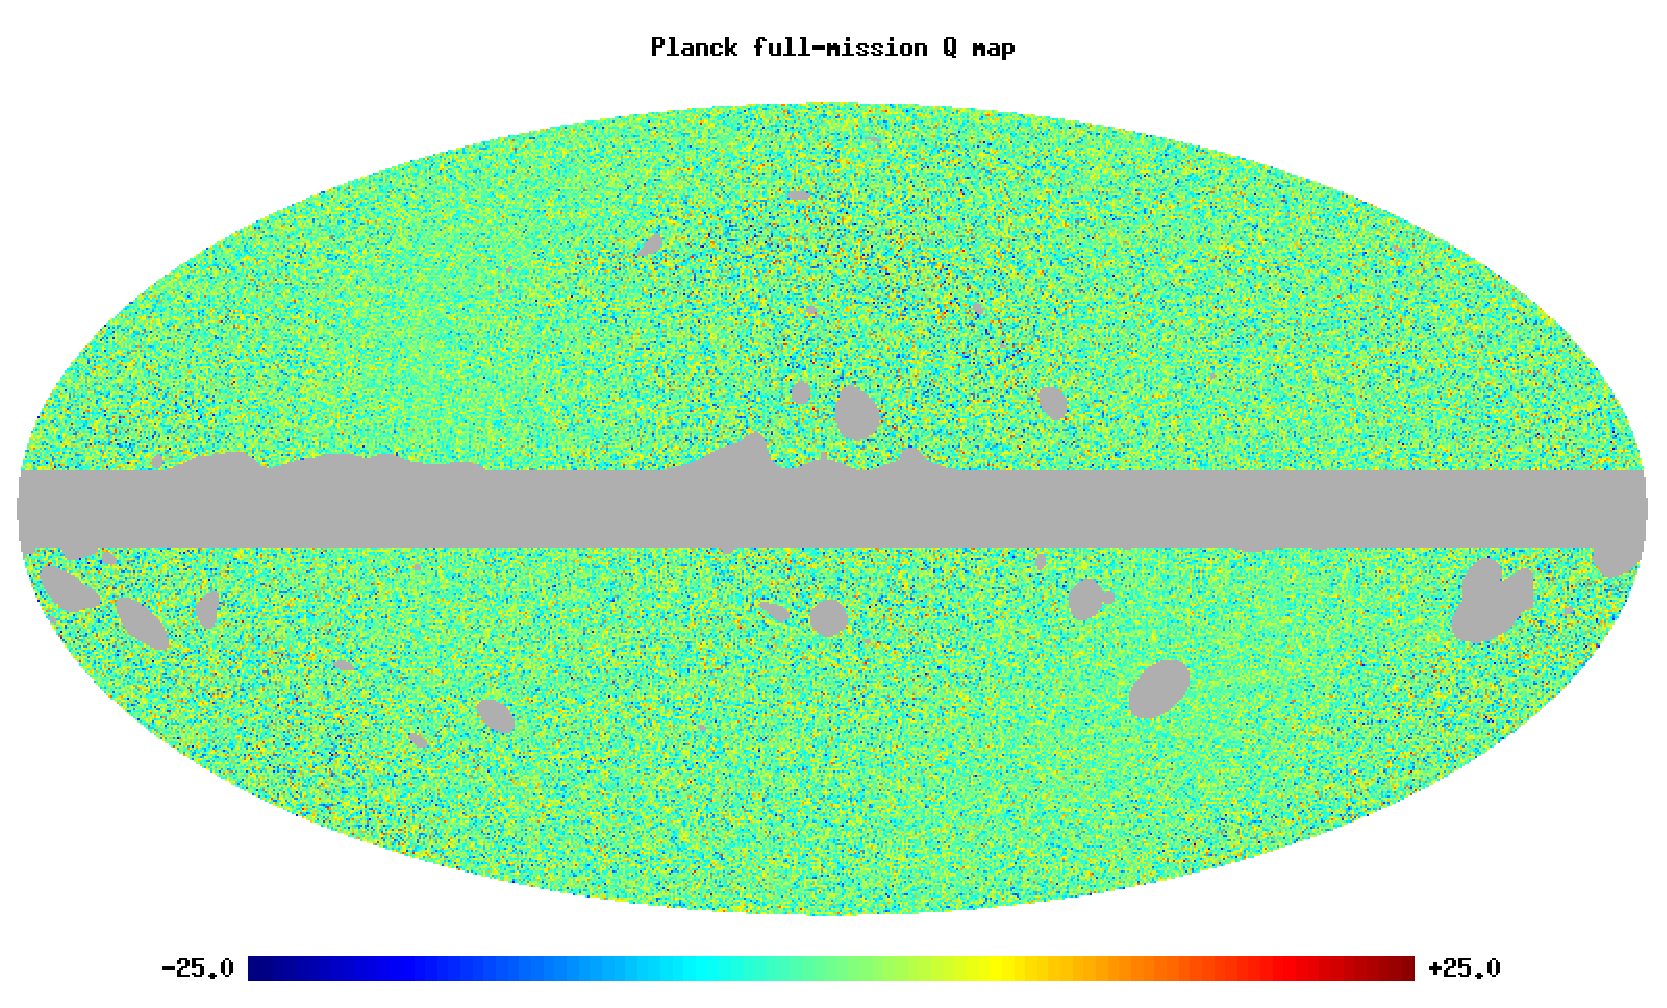
\includegraphics[width=2in]{planckQhp_masked.pdf}
%  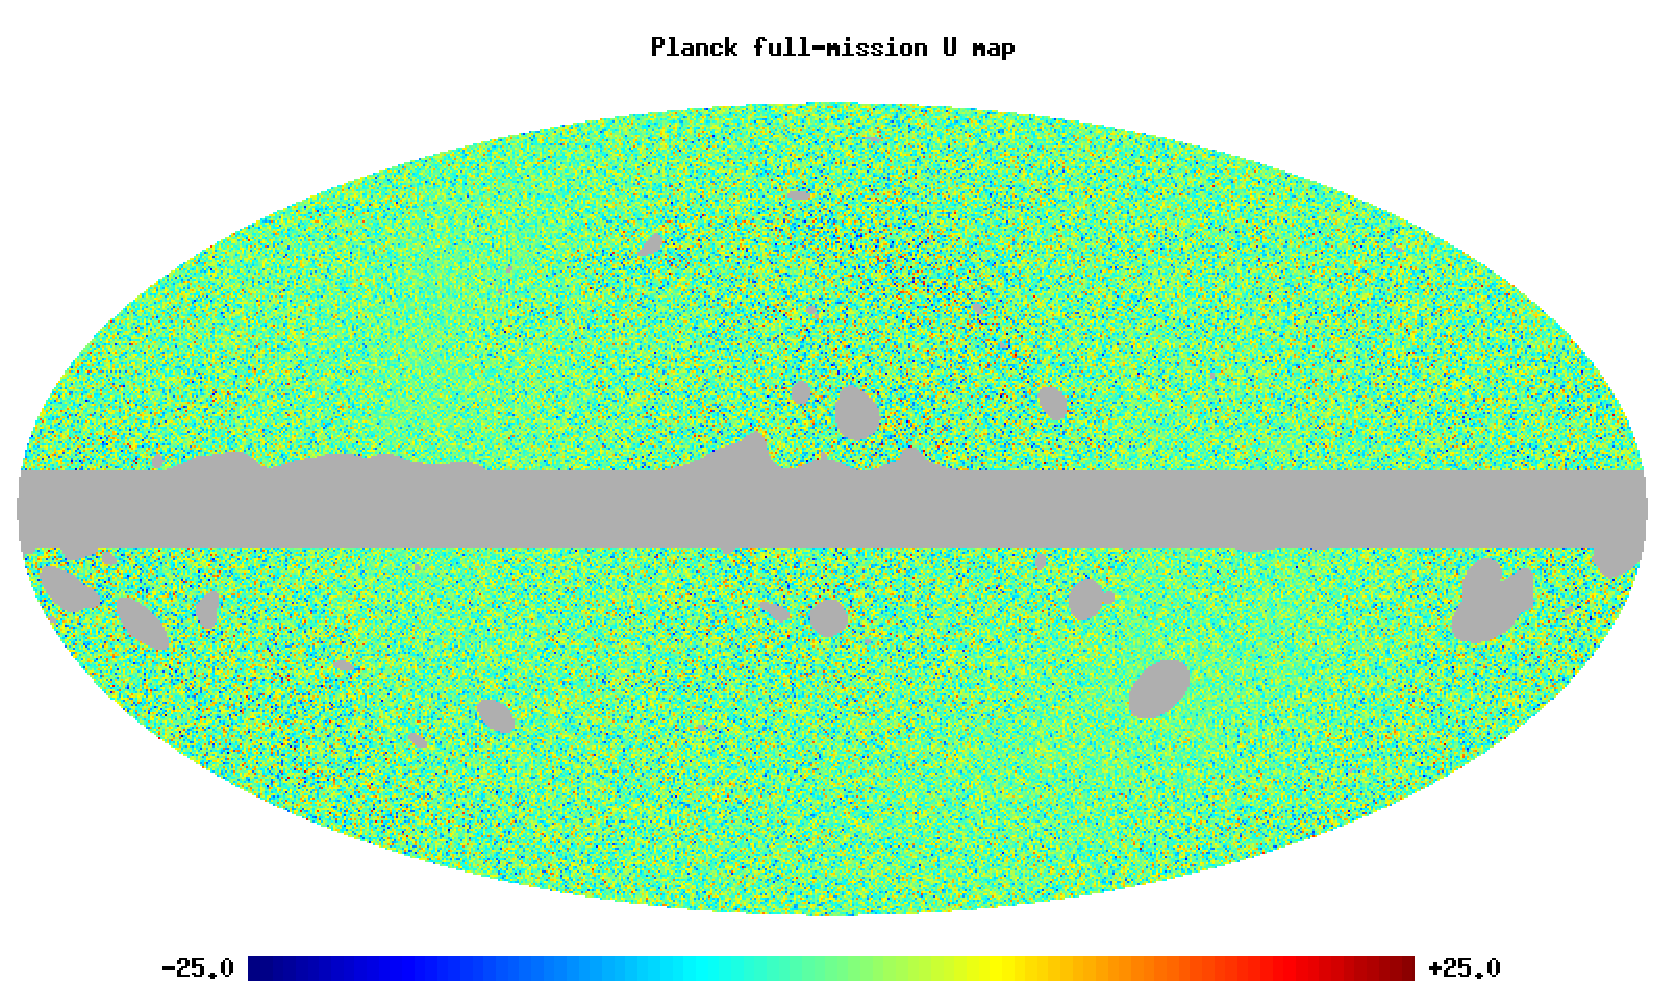
\includegraphics[width=2in]{planckUhp_masked.pdf}  

%  {\hskip 0.2in} {\scriptsize unoriented stacking}     {\hskip 0.65in} {\scriptsize oriented stacking (Bond, Frolov, Huang)}
  
%  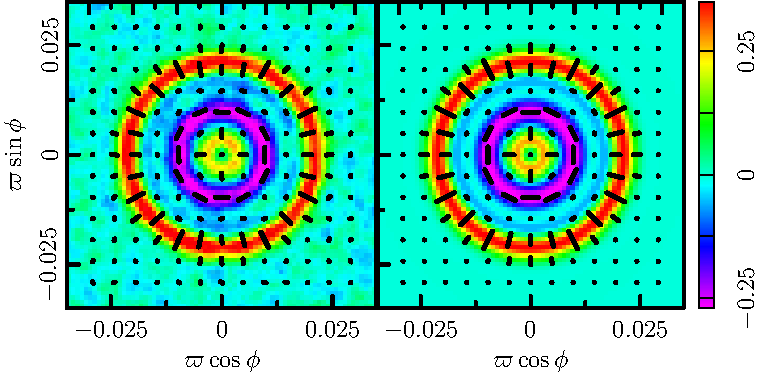
\includegraphics[width=2in]{ors_Qr_on_Tmax_unoriented.pdf}
%  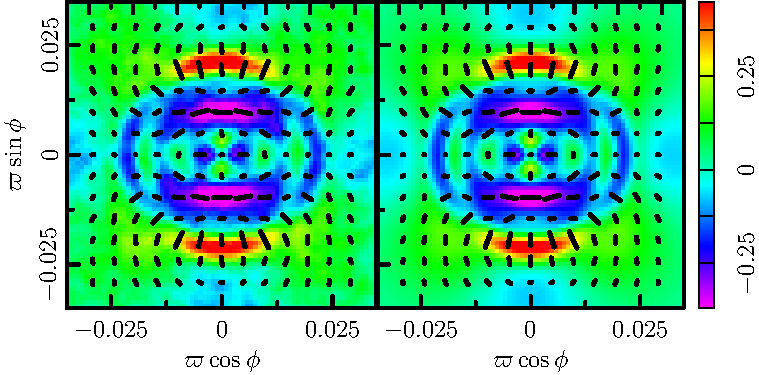
\includegraphics[width=2in]{ors_Q_on_Tmax_oriented.pdf}  
  
%\end{frame}


\begin{frame}
\chtitle{暗物质和暗能量存在的直观证据}
\bch
\hskip 0.2in ACT数据 \hskip 0.6in   标准模型预言

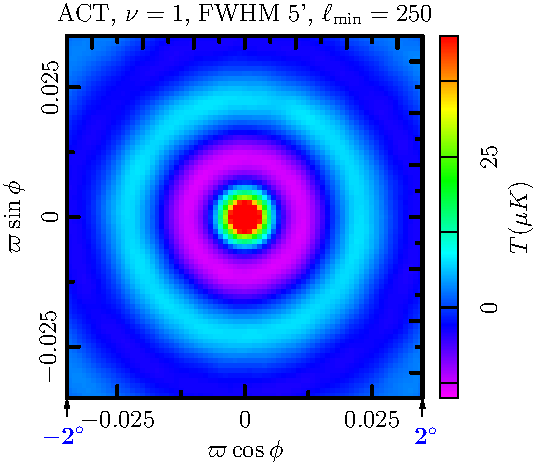
\includegraphics[width=1.3in]{act_T_nu1_5a_lmin250_fpts.pdf}
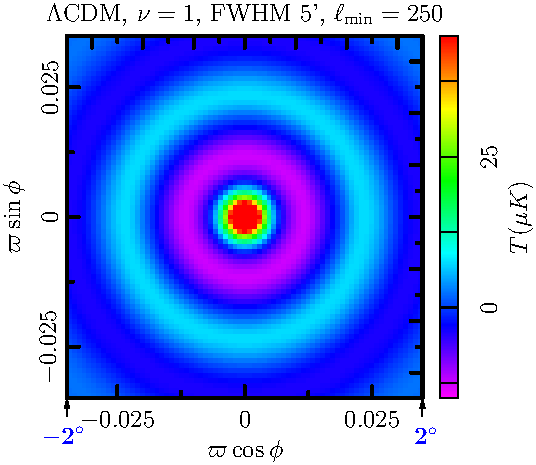
\includegraphics[width=1.3in]{theory_lcdm_T_nu1_5a_lmin250_fpts.pdf}

如果无暗物质 \hskip 0.5in 如果无暗能量
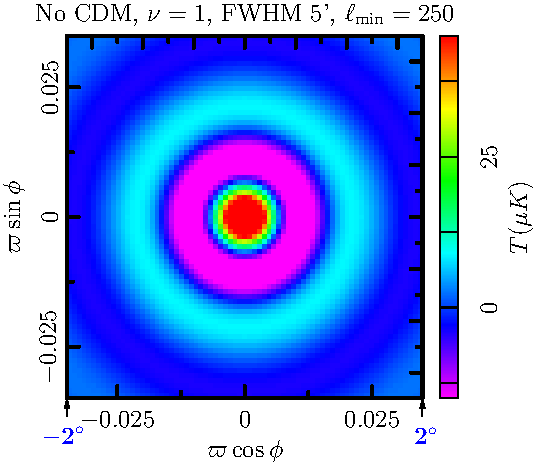
\includegraphics[width=1.3in]{theory_nocdm_T_nu1_5a_lmin250_fpts.pdf}
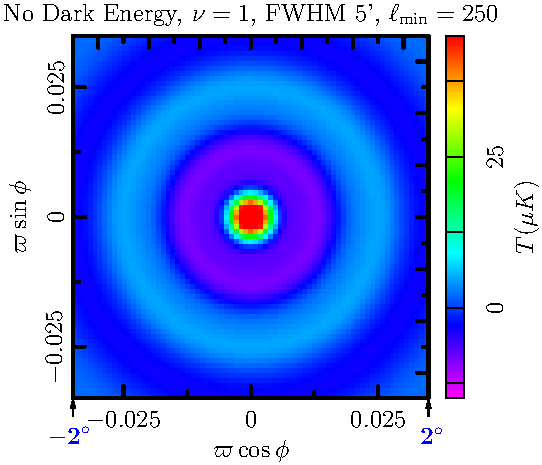
\includegraphics[width=1.3in]{theory_noDE_T_nu1_5a_lmin250_fpts.pdf}

\ech
\end{frame}

\section{Future}

\begin{frame}
\chtitle{宇宙学中还没有解决的问题}
\bch
\begin{itemize}
\item{暗物质粒子的本质是什么?}
\item{暗能量的本质是什么?}
\item{早期宇宙暴涨造成的原初引力波是否能测到?}
\item{能否重建早期宇宙暴涨场的具体粒子物理模型?}
\end{itemize}

这些都是宇宙学里比较热门的研究方向。
\ech
\end{frame}


\begin{frame}
\chtitle{实际的研究往往复杂艰难}

\bch
比如我最近在研究的Horndeski暗能量模型,它的作用量长成这样:
{\scriptsize
  \begin{eqnarray}
    S = && \int \sqrt{-g}d^4x \Big\{ G_2(\phi, X) + G_3(\phi, X)\Box\phi + G_4(\phi,X)R \nonumber \\
    && - 2G_{4,X}(\phi, X)\left[(\Box\phi)^2 - (\nabla^\mu\nabla^\nu\phi) (\nabla_\mu\nabla_\nu\phi)\right] \nonumber \\
    && + G_5(\phi, X)G_{\mu\nu}\nabla^\mu\nabla^\nu\phi +\frac{1}{3}G_{5X}(\phi, X)\times\left[(\Box\phi)^3 \right.\nonumber \\
    && \left.- 3 \Box\phi(\nabla^\mu\nabla^\nu\phi) (\nabla_\mu\nabla_\nu\phi) + 2(\nabla_\mu\nabla_\nu\phi)(\nabla^\sigma\nabla^\nu\phi) (\nabla_\sigma\nabla^\mu\phi)\right]\Big\}\nonumber
  \end{eqnarray}
}
\ech
\end{frame}


\begin{frame}
\chtitle{脑洞大开——未来的命运?}
\bch
如果现在宇宙学标准模型是完全正确的,那么再过个数百亿年宇宙会怎样呢?

\bitem
\item{宇宙继续加速膨胀,银河系将成为宇宙中的孤岛}
\item{人类估计已经灭绝}
\item{那时如果有智能生物出现,他们将不会发现周围有任何其他星系,更无从发现宇宙的加速膨胀}
\item{那时的智能生物掌握的关于宇宙的知识可能永远停留在我们100年前的水平}
  \eitem
\ech
\end{frame}

\begin{frame}
\chtitle{脑洞大开——未来的命运?}
\bch
等等,既然“知识禁锢”是可能的;我们现在的情况有可能已经不妙\wulian
\ech
\end{frame}


\begin{frame}
\chtitle{好了,不能再往下讲了……}
\bch
\skipline
\begin{minipage}{0.4\textwidth}

你再这样讲下去要招不到学生了
\vskip 2in
\ 
\end{minipage}

\includegraphics[width=1.8in]{miaoshu.jpg}
\ech
\end{frame}



\begin{frame}
\chtitle{欢迎报考中山大学}
\addfig{2.5}{spascan.jpg}
\end{frame}


\end{document}



